\chapter{Contexte et objectifs du projet}

\section{Introduction}
Dans ce premier chapitre, nous allons présenter un aperçu global de notre projet. Pour commencer, nous allons décrire l'organisme d'accueil et expliquer le contexte dans lequel notre étude est menée. Ensuite, nous examinerons l'étude de l'existant et exposerons notre proposition de solution. Enfin, nous détaillons notre approche de travail et les outils de gestion de projet que nous allons employer pour mener à bien notre étude.

\section{Présentation de l'organisme d'accueil}
Cette section sera consacrée à la présentation de l'entreprise d'accueil \textbf{IDVEY} où nous avons effectué notre stage de fin d'études.

\subsection{IDVEY}
IDVEY est un cabinet de conseil en transformation digitale basé en Tunisie, fondé en janvier 2018. IDVEY se positionne comme un partenaire stratégique accompagnant les organisations publiques et privées dans leurs projets de transformation numérique.

\begin{figure}[H]
    \centering
    
\includegraphics[width=0.3\linewidth]{img/logo_idvey.png}
    \caption{Logo IDVEY}
    \label{fig:logo-idvey}
\end{figure}

L'entreprise se distingue par son expertise en développement logiciel, intégration de solutions technologiques et conformité réglementaire dans le domaine des services numériques. IDVEY adopte une approche globale qui combine conseil stratégique et exécution technique, permettant ainsi de réduire les frictions liées à la collaboration avec plusieurs prestataires.

\subsection{Domaines d'activité et services}
IDVEY offre une gamme complète de services et de solutions couvrant plusieurs domaines :

\begin{itemize}
    \item \textbf{Conseil et stratégie digitale :} Accompagnement des organisations dans la définition et la mise en œuvre de leur feuille de route de transformation digitale, en tenant compte des aspects stratégiques et opérationnels.

    \item \textbf{Développement web et mobile :} Conception et développement d'applications web et mobiles pour améliorer l'accessibilité et la mobilité des services clients, en utilisant des technologies modernes et des architectures performantes.

    \item \textbf{Intégration de solutions collaboratives :} Support aux organisations dans l'intégration d'outils de collaboration adaptés aux aspects structurels et humains de leurs activités.

    \item \textbf{Solutions e-business (B2B/B2C) :} Développement de plateformes e-commerce cross-platform pour les scénarios B2B et B2C, permettant aux entreprises de développer leur présence en ligne.

    \item \textbf{Gestion de l'information réglementaire (RIM) :} Solutions spécialisées pour les industries, notamment le secteur pharmaceutique (eCTD, sérialisation) et les domaines ESG/retail, garantissant la conformité aux réglementations en vigueur.

    \item \textbf{Business Process Management (BPM) :} Standardisation des flux de travail, automatisation des processus et intégration d'applications pour optimiser les opérations métier.
\end{itemize}

\subsection{Valeurs et approche}
IDVEY s'appuie sur quatre valeurs fondamentales qui guident son action :

\begin{itemize}
    \item \textbf{Engagement :} Implication totale dans la réussite des projets clients.
    \item \textbf{Efficacité :} Optimisation des processus et des solutions pour maximiser les résultats.
    \item \textbf{Confiance :} Construction de relations durables basées sur la transparence et la fiabilité.
    \item \textbf{Innovation :} Adoption des technologies émergentes et des meilleures pratiques du domaine.
\end{itemize}

L'entreprise suit un processus structuré pour garantir la qualité de ses livrables :

\begin{itemize}
    \item \textbf{Conseil et assistance :} Analyse des besoins et définition de la stratégie.
    \item \textbf{Définition des exigences :} Élaboration du cahier des charges détaillé.
    \item \textbf{Conception :} Design et architecture de la solution.
    \item \textbf{Intégration et développement :} Mise en œuvre technique de la solution.
    \item \textbf{Formation et accompagnement :} Support continu et transfert de compétences.
\end{itemize}

IDVEY ne se limite pas à la livraison de solutions techniques, mais accompagne ses clients tout au long du cycle de vie du projet, en accordant une attention particulière aux dimensions humaines et structurelles de la transformation digitale.

\section{Présentation du projet}
Dans cette section, nous décrivons le contexte de notre projet ainsi que la problématique à résoudre. Ensuite, nous exposons de manière claire les objectifs que nous voulons atteindre.

\subsection{Problématique}
La gestion des médicaments représente un défi majeur pour de nombreux patients, particulièrement ceux qui suivent des traitements de longue durée ou souffrent de maladies chroniques. Plusieurs problématiques ont été identifiées :

\begin{itemize}
    \item \textbf{Oubli de la prise des médicaments :} De nombreux patients oublient de prendre leurs médicaments aux heures prescrites, ce qui affecte l'efficacité du traitement et peut entraîner des complications de santé.

    \item \textbf{Gestion complexe des multiples traitements :} Les patients polymorbides ou âgés doivent souvent gérer plusieurs médicaments avec des posologies différentes, ce qui augmente le risque d'erreurs.

    \item \textbf{Suivi des dates de péremption :} La gestion des dates d'expiration des médicaments dans la boîte à pharmacie familiale est souvent négligée, exposant les utilisateurs à des risques sanitaires.

    \item \textbf{Coordination familiale :} Les parents gérant les traitements de leurs enfants ou les aidants s'occupant de personnes âgées manquent d'outils pour coordonner et suivre efficacement les prises de médicaments.

    \item \textbf{Historique et traçabilité :} L'absence d'un système centralisé pour suivre l'historique des traitements rend difficile la communication avec les professionnels de santé.
\end{itemize}

Ces problématiques conduisent à une faible observance thérapeutique, estimée à environ 50\% selon l'Organisation Mondiale de la Santé, avec des conséquences graves sur la santé des patients et une augmentation des coûts de santé.

\subsection{Étude de l'existant}
Dans le cadre de notre analyse approfondie des solutions de gestion des médicaments, nous avons identifié plusieurs applications largement adoptées :

\begin{itemize}
    \item \textbf{Medisafe :} Application mobile de rappel de médicaments avec suivi des prises et alertes. Elle permet de gérer plusieurs traitements mais reste limitée en termes de fonctionnalités collaboratives.

    \item \textbf{MyTherapy :} Solution complète incluant rappels de médicaments, suivi des symptômes et journal de santé. L'interface peut être complexe pour certains utilisateurs, notamment les personnes âgées.

    \item \textbf{Pill Reminder :} Application simple de rappel de médicaments avec interface basique. Manque de fonctionnalités avancées comme la gestion collaborative ou le scan de codes-barres.

    \item \textbf{CareZone :} Plateforme de gestion de santé familiale incluant médicaments, rendez-vous et contacts médicaux. Principalement orientée marché américain avec des fonctionnalités non adaptées au contexte tunisien.
\end{itemize}

\subsection{Critique de l'existant}
Malgré leurs fonctionnalités intéressantes, ces solutions présentent plusieurs limitations :

\begin{itemize}
    \item \textbf{Manque de collaboration efficace :} Les fonctionnalités de gestion familiale sont limitées et ne permettent pas une coordination optimale entre les différents membres de la famille ou les aidants.

    \item \textbf{Absence de gestion de boîte à pharmacie :} Peu de solutions offrent une gestion complète de la boîte à pharmacie avec suivi des quantités, des dates de péremption et des consommations.

    \item \textbf{Interface non adaptée :} Certaines interfaces sont trop complexes pour les personnes âgées ou peu familières avec les technologies.

    \item \textbf{Fonctionnalités limitées en version gratuite :} La plupart des fonctionnalités avancées nécessitent des abonnements payants, limitant l'accessibilité.

    \item \textbf{Manque de système de rôles :} Absence de distinction claire entre gestionnaire, responsable et membre simple dans le cadre familial.
\end{itemize}

\subsection{Solution proposée}
Face à ces constats, nous proposons \textbf{AFYA}, une application mobile complète de gestion des médicaments qui se distingue par :

\begin{itemize}
    \item \textbf{Gestion collaborative avancée :} Système de groupes familiaux avec trois niveaux de rôles (Gestionnaire, Responsable, Membre) permettant une coordination optimale des soins.

    \item \textbf{Boîte à pharmacie intelligente :} Gestion complète des médicaments avec scan de codes-barres/QR, suivi des quantités, alertes de péremption et historique d'achats.

    \item \textbf{Interface intuitive :} Design moderne et ergonomique accessible à tous les utilisateurs, y compris les personnes âgées.

    \item \textbf{Gestion complète des traitements :} Création de traitements avec prescriptions multiples, suivi des doses prises et doses restantes.

    \item \textbf{Système de notifications intelligent :} Rappels personnalisés pour la prise de médicaments, alertes d'expiration, notifications de suivi pour les responsables.

    \item \textbf{Architecture moderne et sécurisée :} Backend Spring Boot avec authentification JWT, application mobile Flutter cross-platform (Android/iOS).
\end{itemize}

La solution AFYA vise à améliorer significativement l'observance thérapeutique tout en facilitant la coordination des soins au sein des familles.

\section{Méthodologie de travail adoptée}
Pour choisir la méthodologie la plus adaptée, il est crucial d'avoir une compréhension approfondie des avantages et des inconvénients de plusieurs options. Dans le cadre de notre projet, nous avons opté pour une approche agile afin d'assurer une meilleure flexibilité et une adaptation continue aux besoins.

\subsection{Les méthodes agiles}
Agile est une philosophie de gestion de projet qui repose sur un ensemble de principes et de valeurs pour aider les équipes de développement à faire face au changement. Les équipes Agile donnent la priorité aux individus et aux interactions plutôt qu'aux processus et aux outils, aux logiciels fonctionnels plutôt qu'à une documentation exhaustive, à la collaboration avec le client plutôt qu'à la négociation des contrats, et à l'adaptation au changement plutôt qu'au suivi strict d'un plan.

Ces valeurs ont été définies dans le Manifeste Agile, ainsi que les 12 principes qui le sous-tendent. Dans Agile, le périmètre du produit est flexible alors que les ressources et les délais sont fixes. Les équipes Agile s'engagent à livrer les logiciels à temps avec l'effectif dont elles disposent.

\subsection{Méthodologie utilisée : Scrum}
Dans le cadre de ce projet, nous avons choisi \textbf{Scrum}, un framework de gestion de projets Agile qui aide les équipes à structurer et à gérer leur travail selon un ensemble de valeurs, de principes et de pratiques.

Scrum encourage les équipes à apprendre par l'expérience, à s'auto-organiser pendant qu'elles tentent de résoudre un problème, mais aussi à réfléchir à leurs victoires et à leurs défaites pour s'améliorer en continu. Même si la méthodologie Scrum est le plus souvent utilisée par les équipes de développement, ses principes et ses enseignements sont valables pour tout type de travail en équipe.

\begin{figure}[H]
    \centering
    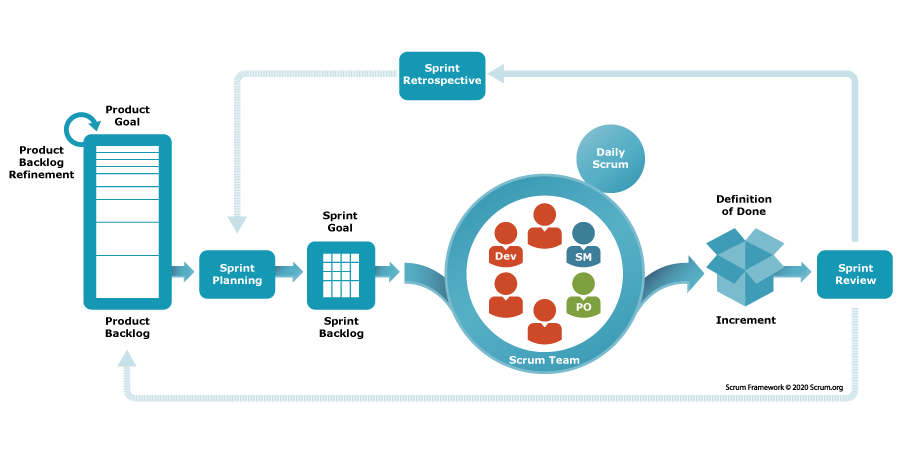
\includegraphics[width=0.8\linewidth]{img/scrum_process.png}
    \caption{Processus Scrum}
    \label{fig:scrum-process}
\end{figure}

\subsubsection{Les différents rôles de la méthodologie Scrum}
La méthodologie Scrum définit trois rôles principaux :

\begin{itemize}
    \item \textbf{Le Product Owner :} Comprend les exigences client et métier, crée et gère le backlog produit en fonction de ces exigences. Il représente l'entreprise et indique les livraisons importantes à l'équipe de développement. Dans notre projet, ce rôle est assuré par l'encadrant professionnel.

    \item \textbf{Le Scrum Master :} S'assure que tout est cohérent et garantit que Scrum fonctionne correctement. Il aide le Product Owner à définir la valeur, l'équipe de développement à fournir de la valeur, et l'équipe Scrum à s'améliorer. C'est un leader-serviteur.

    \item \textbf{L'équipe de développement :} Rassemble les personnes qui réalisent le travail. Dans notre cas, elle comprend le développeur (étudiant) responsable de la conception et du développement de l'application AFYA.
\end{itemize}

\subsubsection{Les événements Scrum}
En Scrum, un projet est organisé en réunions, chacune ayant un objectif précis :

\begin{itemize}
    \item \textbf{Sprint Planning :} Cérémonie qui lance le sprint. Elle a pour objectif de définir ce qui peut être livré dans le sprint et comment y parvenir. Effectuée en collaboration avec toute l'équipe Scrum.

    \item \textbf{Daily Scrum :} Réunion quotidienne de 15 minutes maximum pour discuter de l'avancement et identifier les bloqueurs.

    \item \textbf{Sprint Review :} Marque la fin d'un sprint. L'équipe de développement et les parties prenantes se réunissent pour examiner et présenter le travail accompli pendant le sprint.

    \item \textbf{Sprint Retrospective :} Réunion visant à évaluer le déroulement du dernier sprint, en particulier la dynamique de l'équipe, les processus et les outils, afin d'élaborer un plan d'amélioration.
\end{itemize}

\subsubsection{Les artefacts de Scrum}
Les artefacts Scrum sont des éléments clés permettant de suivre l'avancement du projet :

\begin{itemize}
    \item \textbf{Sprint :} Brève période limitée dans le temps durant laquelle une équipe Scrum effectue une quantité de travail donnée. Notre projet est structuré en 6 sprints.

    \item \textbf{Release :} Correspond à la mise en production d'un ensemble d'incréments validés et testés. Une release peut regrouper plusieurs sprints. Notre projet comporte 3 releases.

    \item \textbf{Product Backlog :} Liste principale des tâches à réaliser, gérée par le Product Owner. C'est une liste dynamique de fonctionnalités, d'exigences, d'améliorations et de correctifs.

    \item \textbf{Sprint Backlog :} Ensemble de tâches du backlog produit sélectionnées pour être développées durant le prochain sprint.

    \item \textbf{Increment :} Livrables créés en exécutant les tâches du backlog produit durant un sprint. Un incrément est toujours compris dans chaque sprint.
\end{itemize}

\section{Présentation du langage de modélisation}
Nous avons choisi \textbf{UML (Unified Modeling Language)} comme langage de modélisation pour notre projet, en raison de sa capacité à décrire visuellement et sémantiquement le fonctionnement et la structure des systèmes logiciels complexes.

Le langage UML a été pensé pour être un langage de modélisation visuelle commun, riche sémantiquement et syntaxiquement. Il est destiné à l'architecture, la conception et la mise en œuvre de systèmes logiciels complexes par leur structure aussi bien que leur comportement.

UML a des applications qui vont au-delà du développement logiciel, notamment pour les flux de processus dans l'industrie. Il ressemble aux plans utilisés dans d'autres domaines et se compose de différents types de diagrammes. Dans l'ensemble, les diagrammes UML décrivent la limite, la structure et le comportement du système et des objets qui s'y trouvent.

\begin{figure}[H]
    \centering
    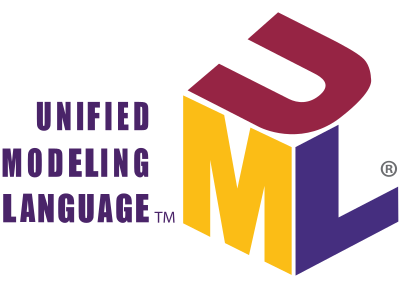
\includegraphics[width=0.4\linewidth]{img/uml_logo.png}
    \caption{Logo UML}
    \label{fig:uml-logo}
\end{figure}

UML 2.0 a apporté plusieurs améliorations :
\begin{itemize}
    \item Une plus grande intégration entre les modèles structurels et comportementaux.
    \item La possibilité de définir une hiérarchie et de décomposer un système logiciel en éléments et sous-éléments.
    \item Le nombre de diagrammes est passé de 9 à 13, offrant plus de flexibilité dans la modélisation.
\end{itemize}

Dans notre projet, nous utiliserons principalement les diagrammes de cas d'utilisation, de classes et de séquence pour modéliser l'application AFYA.

\section{Conclusion}
Dans ce premier chapitre, nous avons présenté le contexte du projet AFYA, en commençant par la présentation de l'organisme d'accueil IDVEY. Nous avons ensuite exposé la problématique de la gestion des médicaments et analysé les solutions existantes avec leurs limites. Notre solution proposée, l'application AFYA, apporte des réponses concrètes aux problèmes identifiés grâce à une approche collaborative et des fonctionnalités avancées.

Nous avons également justifié le choix de la méthodologie Agile Scrum pour la gestion du projet, en détaillant ses différents rôles, événements et artefacts. Enfin, nous avons présenté UML comme langage de modélisation pour la conception de notre système.

Le chapitre suivant nous permettra d'analyser et de spécifier en détail les besoins fonctionnels et non fonctionnels du projet AFYA.
